\chapter{Diffraction de Fraunhofer et filtrage spatial}\label{ch:b2:diffraction}

Plissez les yeux vers un réverbère à travers l'interstice entre deux doigts et le
lampadaire s'étire en une bande de franges~; regardez une étoile dans la
meilleure lunette et vous ne voyez pas un point mais un petit disque cerné de
cercles pâles. La lumière qui passe par une ouverture s'étale --- plus
l'ouverture est étroite, plus l'étalement est large --- et aucune lentille ne peut la focaliser
plus serré que cet étalement ne l'autorise. C'est la \emph{\omterm{def:b2:diffraction:huygens}{diffraction}}, la raison pour laquelle
un microscope ne peut voir un virus, le pouvoir de résolution d'une lunette croît
avec son diamètre, et un faisceau laser ne peut rester parallèle. Ce chapitre
calcule la figure de \omterm{def:b2:diffraction:huygens}{diffraction} d'une ouverture en champ lointain, la
limite qu'elle impose à tout instrument d'optique, la façon dont elle se combine à
l'interférence, et l'idée --- celle d'Abbe --- qui fait du plan focal d'une
lentille un lieu où l'on peut filtrer une image.

\section{Le principe de Huygens--Fresnel et le régime de Fraunhofer}

\begin{definition}[Principe de Huygens--Fresnel]\label{def:b2:diffraction:huygens}
\index{principe de Huygens--Fresnel}\index{diffraction}\index{diffraction de Fraunhofer}
Tout point d'un front d'onde (ou d'une ouverture éclairée par une onde) agit comme une
source secondaire émettant une ondelette sphérique, en phase avec l'onde
en ce point~; l'onde au-delà est la somme cohérente des ondelettes. Pour une
ouverture $\Sigma$ éclairée par une onde plane d'amplitude $a$, l'amplitude
parvenant en un point lointain vaut $\underline s(M) = K\iint_\Sigma\eu^{-\iu\varphi(P, M)}\dd S$, avec
$\varphi(P, M)$ la phase du trajet du point $P$ de l'ouverture jusqu'à $M$
($K$ une constante). La diffraction de \emph{Fraunhofer} (champ lointain) est le cas
où $M$ est à l'infini --- ou dans le plan focal d'une lentille --- de sorte que
les rayons issus de tous les points de l'ouverture vers $M$ sont parallèles, dans
la direction $\vect u$, et
\[
\varphi(P, M) = \varphi_0 - \frac{2\pi}\lambda\,\vect{OP}\cdot\vect u , \qquad
\underline s(\vect u) \propto \iint_\Sigma\eu^{\iu(2\pi/\lambda)\vect{OP}\cdot\vect u}\dd S .
\]
La figure s'observe à l'infini, ou au foyer $F'$ d'une lentille,
où la direction $\vect u$ de petits angles $(\alpha, \beta)$ correspond au
point $(f\alpha, f\beta)$.
\end{definition}
\admitted

\begin{remark}[Assez loin~?]\label{rem:b2:diffraction:fresnelnumber}
\index{nombre de Fresnel}
Pour une ouverture de taille $D$ vue à la distance $L$ sans lentille, les
rayons sont assez parallèles quand le terme quadratique de
l'\cref{exo:b2:scalar-light-model:12} est négligeable, $D^2/L \ll \lambda$ ---
le \emph{\omterm{rem:b2:diffraction:fresnelnumber}{nombre de Fresnel}} $D^2/\lambda L \ll 1$. Une fente de \qty{0.1}{mm} à
\qty{500}{nm} demande $L \gg \qty{2}{cm}$~; une ouverture de \qty{1}{cm}, $L \gg \qty{200}{m}$ ---
d'où la lentille, qui ramène l'infini dans son plan focal. Plus près
(\omterm{def:b2:diffraction:huygens}{diffraction} de Fresnel) les figures sont plus complexes~; l'ombre d'un
bord droit, par exemple, porte des franges du côté éclairé.
\end{remark}

\section{La fente unique et l'ouverture circulaire}

\begin{proposition}[Diffraction par une fente]\label{prop:b2:diffraction:slit}
\index{diffraction par une fente}\index{fonction sinus cardinal}
Une fente de largeur $b$ (longue selon $y$) éclairée sous incidence normale envoie dans
la direction $\theta$ (dans le plan perpendiculaire à la fente)
l'intensité
\[
I(\theta) = I_0\,\operatorname{sinc}^2\Bigl(\frac{\pi b\sin\theta}\lambda\Bigr) , \qquad \operatorname{sinc}x = \frac{\sin x}x :
\]
un maximum central brillant de demi-largeur angulaire $\lambda/b$ (premiers zéros en
$\sin\theta = \pm\lambda/b$), contenant $90\%$ de la lumière, et des maxima secondaires
vers $\sin\theta = \pm1.43\lambda/b$, $\pm2.46\lambda/b$, \dots, d'intensités
relatives $4.7\%$, $1.6\%$, \dots --- plus la fente est étroite, plus
la figure est large. Dans le plan focal d'une lentille de distance focale $f$, le
maximum central est large de $2\lambda f/b$.
\end{proposition}

\begin{proof}
$\underline s(\theta) \propto \int_{-b/2}^{b/2}\eu^{\iu kx\sin\theta}\dd x = b\,\operatorname{sinc}(kb\sin\theta/2)$
avec $k = 2\pi/\lambda$~; élever au carré. Zéros là où $b\sin\theta = m\lambda$, $m \ne 0$~: les
ondelettes des deux moitiés de la fente s'annulent alors deux à deux.
\end{proof}

\begin{omfigure}
\begin{tikzpicture}[font=\small, x=1cm, y=1cm, >=Stealth]
  \begin{scope}
    \draw[thick] (0,-2) -- (0,-0.5) (0,0.5) -- (0,2);
    \draw[<->] (-0.35,-0.5) -- (-0.35,0.5) node[midway, left, font=\footnotesize] {$b$};
    \foreach \y in {-1.6,-0.9,-0.2,0.5,1.2} \draw[omDef, ->] (-2.2,\y) -- (-0.1,\y);
    \foreach \y in {-0.4,-0.2,0,0.2,0.4} \draw[omThm, thick, ->] (0.1,\y) -- (2.4,{\y+1.0});
    \draw[dashed] (0.1,0) -- (2.6,0); \draw (1.4,0) arc[start angle=0, end angle=23.5, radius=1.4]; \node[font=\footnotesize] at (1.7,0.28) {$\theta$};
    \node[font=\footnotesize] at (1.2,-1.6) {$b\sin\theta = \lambda$: premier zéro};
  \end{scope}
  \begin{scope}[xshift=8.6cm]
    \begin{axis}[omaxis, axis x line=bottom, axis y line=left, width=6.4cm, height=4.4cm, at={(0,-2.0cm)},
        xlabel={$b\sin\theta/\lambda$}, ylabel={$I/I_0$}, xmin=-3.2, xmax=3.2, ymin=0, ymax=1.1, xtick={-3,-2,-1,0,1,2,3}, ytick={0.5,1}, samples=400,
        xlabel style={at={(axis description cs:0.5,-0.14)}, anchor=north},
        ylabel style={at={(axis description cs:-0.1,0.5)}, rotate=90, anchor=south}]
      \addplot[omDef, thick, domain=-3.2:3.2] {(sin(deg(pi*x))/(pi*x+1e-9))^2};
    \end{axis}
  \end{scope}
\end{tikzpicture}

{\small À gauche~: les ondelettes issues de toute la fente, sommées dans la direction
$\theta$. À droite~: la figure de Fraunhofer de la fente, en $\operatorname{sinc}^2$~: un
lobe central deux fois plus large que les autres et bien plus brillant.}
\end{omfigure}

\begin{proposition}[Ouverture circulaire~; la tache d'Airy]\label{prop:b2:diffraction:airy}
\index{tache d'Airy}\index{critère de Rayleigh (résolution)}\index{pouvoir de résolution (instrument)}
Une ouverture circulaire de diamètre $D$ donne un disque central brillant, la
\emph{\omterm{prop:b2:diffraction:airy}{tache d'Airy}}, entourée d'anneaux pâles~; le premier anneau sombre est en
\[
\sin\theta = 1.22\,\frac\lambda D ,
\]
et la tache retient $84\%$ de la lumière. Tout instrument dont la
pupille d'entrée a le diamètre $D$ --- œil, appareil photo, télescope, objectif
de microscope --- transforme une source ponctuelle en une \omterm{prop:b2:diffraction:airy}{tache d'Airy} de ce rayon
angulaire~; deux points sont \emph{résolus} (critère de Rayleigh) si leur
séparation angulaire dépasse $1.22\lambda/D$~: c'est le pouvoir de résolution de
l'instrument.
\end{proposition}
\admitted

\begin{example}[Œil, télescope, microscope]\label{ex:b2:diffraction:instruments}
L'œil ($D = \qty{3}{mm}$, $\lambda = \qty{550}{nm}$)~: $1.22\lambda/D = \qty{2.2e-4}{rad}$, environ
\qty{45}{''} --- un détail de \qty{1}{mm} à \qty{4}{m}, ce qui est bien à peu près
l'acuité d'un bon œil~: l'évolution a accordé les cellules de la rétine à la
limite de \omterm{def:b2:diffraction:huygens}{diffraction}. Un télescope de \qty{2.4}{m}~: \qty{0.06}{''}, mille fois
mieux, si l'atmosphère le permet (elle ne le permet pas, depuis le sol~:
\qty{1}{''} de «~seeing~», d'où les télescopes spatiaux et l'optique adaptative). Une
antenne radio de \qty{100}{m} à $\lambda = \qty{21}{cm}$~: \qty{9}{'}, moins bien que l'œil~;
les interféromètres à l'échelle des continents restaurent la résolution. Un
objectif de microscope d'angle d'ouverture $\alpha$ résout $0.61\lambda/n\sin\alpha$
--- environ \qty{0.2}{\micro m} dans le visible, quel que soit le grandissement~: la
limite qui a poussé la microscopie vers les électrons et les rayons X.
\end{example}

\begin{omfigure}
\begin{tikzpicture}[font=\small, x=1cm, y=1cm]
  \begin{scope}
    \foreach \r/\g in {1.5/85, 1.25/70, 1.0/50, 0.8/25, 0.6/5, 0.45/40, 0.3/70, 0.15/95} {
      \fill[black!\g] (0,0) circle (\r);
    }
    \node[font=\footnotesize] at (0,-1.9) {figure d'Airy d'une étoile};
  \end{scope}
  \begin{scope}[xshift=4.2cm]
    \foreach \r/\g in {0.8/25, 0.6/5, 0.45/40, 0.3/70, 0.15/95} {
      \fill[black!\g] (-0.45,0) circle (\r);
    }
    \foreach \r/\g in {0.8/25, 0.6/5, 0.45/40, 0.3/70, 0.15/95} {
      \fill[black!\g, opacity=0.6] (0.45,0) circle (\r);
    }
    \node[font=\footnotesize] at (0,-1.9) {deux étoiles à la limite de Rayleigh};
  \end{scope}
  \begin{scope}[xshift=9.6cm]
    \begin{axis}[omaxis, axis x line=bottom, axis y line=left, width=5.4cm, height=4.0cm, at={(0,-1.8cm)},
        xlabel={$\theta D/\lambda$}, ylabel={$I$}, xmin=-2.5, xmax=3.5, ymin=0, ymax=1.5, xtick={-1.22,0,1.22,2.44}, xticklabels={$-1.22$,$0$,$1.22$,$2.44$}, ytick=\empty, samples=300,
        xlabel style={at={(axis description cs:0.5,-0.14)}, anchor=north},
        ylabel style={at={(axis description cs:-0.06,0.5)}, rotate=90, anchor=south}]
      \addplot[omDef, thick, domain=-2.5:3.5] {(sin(deg(pi*x/1.22))/(pi*x/1.22+1e-9))^2};
      \addplot[omThm, thick, domain=-2.5:3.5] {(sin(deg(pi*(x-1.22)/1.22))/(pi*(x-1.22)/1.22+1e-9))^2};
    \end{axis}
  \end{scope}
\end{tikzpicture}

{\small À gauche et au milieu~: la \omterm{prop:b2:diffraction:airy}{tache d'Airy} d'une source ponctuelle, et deux
sources à la limite de Rayleigh --- le centre de l'une sur le premier anneau
sombre de l'autre. À droite~: leurs profils (esquissés par des formes en
$\operatorname{sinc}^2$), séparés de $1.22\lambda/D$.}
\end{omfigure}

\section{Diffraction et interférence ensemble}

\begin{proposition}[Fentes d'Young de largeur finie~; l'enveloppe du réseau]\label{prop:b2:diffraction:combined}
\index{enveloppe (diffraction)}\index{ordres manquants}
Deux fentes de largeur $b$ dont les centres sont distants de $a$ donnent
\[
I(\theta) = 4I_0\,\operatorname{sinc}^2\Bigl(\frac{\pi b\sin\theta}\lambda\Bigr)\cos^2\Bigl(\frac{\pi a\sin\theta}\lambda\Bigr) :
\]
les franges d'Young (de pas $\lambda/a$ en $\sin\theta$) sous l'enveloppe de la
fente seule (de largeur $2\lambda/b$)~; $a/b$ franges remplissent le lobe central, et les
franges en $a\sin\theta = p\lambda$ qui tombent sur un zéro de l'enveloppe
($b\sin\theta = m\lambda$) sont \emph{manquantes}. Un réseau de $N$ fentes de largeur
$b$ a de même ses maxima principaux modulés par la même enveloppe ---
que le blaze du \cref{ch:b2:gratings} incline vers l'ordre utilisé.
\end{proposition}

\begin{proof}
L'intégrale sur l'ouverture se scinde en une somme, sur les deux fentes, de la même
intégrale décalée de $\pm a/2$~: $\underline s \propto b\,\operatorname{sinc}(\pi b\sin\theta/\lambda)
\times2\cos(\pi a\sin\theta/\lambda)$. Pour $N$ fentes le second facteur est la
somme à $N$ ondes.
\end{proof}

\begin{omfigure}
\begin{tikzpicture}
\begin{axis}[omaxis, axis x line=bottom, axis y line=left, width=13.6cm, height=4.6cm,
    xlabel={$a\sin\theta/\lambda$}, ylabel={$I/4I_0$}, xmin=-9, xmax=9, ymin=0, ymax=1.1, xtick={-8,-4,0,4,8}, ytick={0.5,1}, samples=1200,
    xlabel style={at={(axis description cs:0.5,-0.12)}, anchor=north},
    ylabel style={at={(axis description cs:-0.04,0.5)}, rotate=90, anchor=south}]
  \addplot[omDef, thick, domain=-9:9] {(sin(deg(pi*x/4))/(pi*x/4+1e-9))^2*cos(deg(pi*x))^2};
  \addplot[omThm, thick, dashed, domain=-9:9] {(sin(deg(pi*x/4))/(pi*x/4+1e-9))^2};
\end{axis}
\end{tikzpicture}

{\small Deux fentes avec $a = 4b$~: les franges d'Young sous l'enveloppe de la
fente seule (tiretée)~; les franges du quatrième ordre tombent sur les zéros de
l'enveloppe et manquent.}
\end{omfigure}

\section{Le plan de Fourier et le filtrage spatial}

\begin{proposition}[La lentille comme analyseur de Fourier]\label{prop:b2:diffraction:fourier}
\index{plan de Fourier}\index{fréquence spatiale}\index{filtrage spatial}\index{théorie d'Abbe}
Un transparent de transmittance $t(x, y)$ dans le plan focal objet d'une
lentille, éclairé par une onde plane, produit dans le plan focal image
l'amplitude
\[
\underline s(X, Y) \propto \iint t(x, y)\,\eu^{-\iu2\pi(xX + yY)/\lambda f}\dd x\,\dd y
\]
--- sa transformée de Fourier à deux dimensions, chaque point $(X, Y)$ du
\emph{\omterm{prop:b2:diffraction:fourier}{plan de Fourier}} recueillant la lumière diffractée sous les angles
$(X/f, Y/f)$, c'est-à-dire les \emph{\omterm{prop:b2:diffraction:fourier}{fréquences spatiales}} $(X/\lambda f, Y/\lambda f)$ de
l'objet~: les détails fins (hautes fréquences) loin de l'axe, les grossiers
près de lui. Une seconde lentille reforme l'image à partir de ce plan~; tout ce
qui y est bloqué ou modifié est filtré hors de l'image
(\emph{\omterm{prop:b2:diffraction:fourier}{filtrage spatial}}, \omterm{prop:b2:diffraction:fourier}{théorie d'Abbe} du microscope)~: un trou d'aiguille
sur l'axe ne garde que les basses fréquences (lissage, «~nettoyage~» d'un
faisceau laser)~; un cache sur l'axe supprime le fond uniforme et
garde les bords (fond noir, strioscopie)~; une \omterm{prop:b2:plane-waves-polarization:plates}{lame quart d'onde} sur
l'axe transforme les objets de phase, invisibles autrement, en contraste d'intensité
(contraste de phase, Zernike).
\end{proposition}

\begin{proof}[Justification]
Dans l'intégrale de Fraunhofer, $\vect{OP}\cdot\vect u = x\alpha + y\beta$ avec la
direction associée à $(X, Y) = (f\alpha, f\beta)$~; la transmittance pondère
chaque source secondaire. (La transformation de Fourier elle-même est étudiée dans le
volume de mathématiques de troisième année~; ici, ce n'est que le nom de cette intégrale.)
Pour un objet périodique de période $d$, la transformée est l'ensemble des ordres du
réseau en $X = p\lambda f/d$~: l'image ne peut montrer la période que si au moins
les ordres $\pm1$ traversent la lentille --- la condition d'Abbe, qui est de nouveau
la limite de résolution du microscope.
\end{proof}

\begin{omfigure}
\begin{tikzpicture}[font=\small, x=1cm, y=1cm, >=Stealth]
  \draw[omDef, thick, ->] (-5.6,0.8) -- (-4.6,0.8); \draw[omDef, thick, ->] (-5.6,0) -- (-4.6,0); \draw[omDef, thick, ->] (-5.6,-0.8) -- (-4.6,-0.8);
  \draw[thick, fill=omExo!20] (-4.4,-1.4) rectangle (-4.3,1.4); \node[font=\footnotesize] at (-4.35,-1.75) {objet $t(x, y)$};
  \draw[thick, fill=omExo!20] (-2.4,0) ellipse (0.2 and 1.5); \node[font=\footnotesize] at (-2.4,-1.85) {$L_1$};
  \draw[thick] (0,-1.4) -- (0,1.4); \fill[omThm] (0,0) circle (2pt); \fill[omThm] (0,0.7) circle (1.5pt); \fill[omThm] (0,-0.7) circle (1.5pt);
  \node[font=\footnotesize] at (0,-1.75) {plan de Fourier};
  \draw[thick, fill=omExo!20] (2.4,0) ellipse (0.2 and 1.5); \node[font=\footnotesize] at (2.4,-1.85) {$L_2$};
  \draw[thick, fill=omExo!20] (4.3,-1.4) rectangle (4.4,1.4); \node[font=\footnotesize] at (4.35,-1.75) {image};
  \draw[omThm] (-4.35,0.6) -- (-2.4,1.0) -- (0,0.7) -- (2.4,0.4) -- (4.35,-0.6);
  \draw[omThm] (-4.35,-0.6) -- (-2.4,-1.0) -- (0,-0.7) -- (2.4,-0.4) -- (4.35,0.6);
  \draw[omProp] (-4.35,0.6) -- (-2.4,0.6) -- (0,0) -- (2.4,-0.6) -- (4.35,-0.6);
  \draw[omProp] (-4.35,-0.6) -- (-2.4,-0.6) -- (0,0) -- (2.4,0.6) -- (4.35,0.6);
  \draw[<->] (-4.35,1.7) -- (-2.4,1.7) node[midway, above, font=\footnotesize] {$f$}; \draw[<->] (-2.4,1.7) -- (0,1.7) node[midway, above, font=\footnotesize] {$f$};
  \node[omThm, font=\footnotesize, anchor=west] at (0.15,0.95) {ordres d'un objet périodique};
\end{tikzpicture}

{\small Le montage $4f$~: la première lentille forme la transformée de Fourier
de l'objet dans son plan focal (un objet périodique y donne des
ordres discrets), la seconde reforme l'image~; un masque dans le
\omterm{prop:b2:diffraction:fourier}{plan de Fourier} filtre l'image.}
\end{omfigure}

\begin{example}[Nettoyer un faisceau, voir l'invisible]\label{ex:b2:diffraction:filtering}
Un faisceau laser porte poussières et rides~: focalisez-le à travers un trou de
quelques micromètres --- la taille de la \omterm{prop:b2:diffraction:airy}{tache d'Airy} centrale du faisceau
gaussien propre --- et tout le reste, qui tombe à l'extérieur, est bloqué~;
le faisceau recollimaté est lisse~: c'est un \emph{filtre spatial}. Une cellule
vivante est transparente~; elle ne change que la phase de la lumière. Bloquer
la tache axiale rend ses bords brillants sur fond noir~; la lame de Zernike
décale la lumière non diffractée d'un quart d'onde afin qu'elle interfère
en intensité avec la lumière diffractée~: l'intérieur de la cellule apparaît,
et la biologie a eu son microscope (prix Nobel 1953).
\end{example}

\begin{method}[Estimations de diffraction]\label{met:b2:diffraction:method}
(1) Étalement angulaire $\sim\lambda/b$ pour une ouverture de taille $b$ ($1.22\lambda/D$ pour
un cercle)~; la taille de la figure à la distance $L$ ou à la distance focale $f$ vaut
$\lambda L/b$, $\lambda f/b$. (2) Vérifier la condition de Fraunhofer $b^2/\lambda L \ll 1$ ou
utiliser une lentille. (3) Combiner~: enveloppe de \omterm{def:b2:diffraction:huygens}{diffraction} $\times$ franges
d'interférence. (4) Résolution~: deux points demandent $\Delta\theta > 1.22\lambda/D$~; un objet
périodique demande que ses premiers ordres entrent dans la pupille. (5) L'image du \omterm{prop:b2:diffraction:fourier}{plan
de Fourier}~: quoi bloquer pour ôter quel détail.
\end{method}

\section{Exercices}

\begin{exercise}[$\star$]\label{exo:b2:diffraction:1}
Une fente de \qty{0.10}{mm} éclairée par un laser He--Ne (\qty{633}{nm})~; écran à
\qty{2.0}{m}. Largeur du maximum central~; position des deux premiers
maxima secondaires~; \omterm{rem:b2:diffraction:fresnelnumber}{nombre de Fresnel} --- l'écran est-il assez loin~? Même
fente avec une lentille de $f = \qty{50}{cm}$.
\end{exercise}

\begin{exercise}[$\star$]\label{exo:b2:diffraction:2}
Pouvoir de résolution (Rayleigh) de~: l'œil (\qty{3}{mm}, \qty{550}{nm})~; une
lunette d'amateur de \qty{10}{cm}~; le miroir de \qty{2.4}{m} de Hubble~; une antenne
radio de \qty{64}{m} à \qty{6}{cm}~; un objectif photo de \qty{50}{mm} à $f/8$ (pupille \qty{6}{mm})~:
taille de la \omterm{prop:b2:diffraction:airy}{tache d'Airy} sur le capteur, comparée à un pixel de \qty{4}{\micro m}.
\end{exercise}

\begin{exercise}[$\star$]\label{exo:b2:diffraction:3}
Deux fentes de largeur $b = \qty{0.05}{mm}$, centres distants de $a = \qty{0.25}{mm}$, $\lambda =
\qty{500}{nm}$, lentille $f = \qty{1}{m}$~: interfrange~; largeur de l'enveloppe
centrale~; nombre de franges qu'elle contient~; quels ordres manquent~?
\end{exercise}

\begin{exercise}[$\star$]\label{exo:b2:diffraction:4}
Un faisceau laser de \qty{2}{mm} de diamètre à \qty{633}{nm} se propage jusqu'à la Lune
(\qty{3.8e8}{m})~: angle de \omterm{def:b2:diffraction:huygens}{diffraction} $\sim1.22\lambda/D$, diamètre de la tache~;
avec un télescope de \qty{3.5}{m} comme émetteur~; pourquoi les retours de télémétrie lunaire sont-ils si
faibles (le rétroréflecteur, \qty{1}{m}, renvoie la lumière avec sa propre
\omterm{def:b2:diffraction:huygens}{diffraction})~?
\end{exercise}

\begin{exercise}[$\star\star$]\label{exo:b2:diffraction:5}
\emph{La fente en détail.} (a) Mener l'intégrale de Fraunhofer pour
la fente et obtenir $\operatorname{sinc}^2$. (b) Montrer que les maxima secondaires
sont en $\tan x = x$ ($x = \pi b\sin\theta/\lambda$), le premier près de $x = 1.43\pi$, et
calculer son intensité relative. (c) Fraction de l'énergie dans le
lobe central (on admet $\int_{-\pi}^\pi\operatorname{sinc}^2 = 0.903\pi$ et
$\int_{-\infty}^\infty\operatorname{sinc}^2 = \pi$). (d) La fente est éclairée sous l'incidence
$\theta_0$~: montrer que la figure est la même, centrée sur la direction $\theta_0$.
\end{exercise}

\begin{exercise}[$\star\star$]\label{exo:b2:diffraction:6}
\emph{Microscope.} Un objectif d'\omterm{prop:b2:guided-waves:fibre}{ouverture numérique} $n\sin\alpha = 1.4$
(immersion à huile) à \qty{500}{nm}~: plus petite distance résolue $0.61\lambda/n\sin
\alpha$~; en lumière bleue (\qty{400}{nm})~; dans l'ultraviolet (\qty{250}{nm})~; pourquoi
un oculaire $1000\times$ n'aide-t-il pas (la limite propre de l'œil à \qty{25}{cm} est
\qty{0.1}{mm})~? Que changent les microscopes électroniques ($\lambda = \qty{4}{pm}$ à
\qty{100}{keV})~?
\end{exercise}

\begin{exercise}[$\star\star$]\label{exo:b2:diffraction:7}
\emph{Rectangulaire et circulaire.} (a) Une ouverture rectangulaire $b \times h$~:
montrer que la figure est $\operatorname{sinc}^2(\pi b\sin\theta_x/\lambda)\operatorname{sinc}^2(\pi h
\sin\theta_y/\lambda)$~: une croix, plus large selon le côté le plus étroit. (b) Un carré de
\qty{0.2}{mm} avec $f = \qty{1}{m}$~: taille du carré central. (c) Pour un
cercle de même largeur le premier zéro est en $1.22\lambda/D$ au lieu de $\lambda/b$~:
pourquoi plus loin (penser à la lumière concentrée près du centre d'un
disque)~? (d) Le miroir secondaire d'un télescope est tenu par quatre bras~:
qu'ajoutent-ils à l'image d'une étoile brillante~?
\end{exercise}

\begin{exercise}[$\star\star$]\label{exo:b2:diffraction:8}
\emph{Abbe.} Un réseau de pas $d = \qty{2}{\micro m}$ est observé avec un
objectif de microscope d'angle d'ouverture $\alpha$ dans l'air, $\lambda = \qty{550}{nm}$.
(a) Angles de ses ordres $\pm1$, $\pm2$. (b) $\sin\alpha$ minimal pour que l'image
montre la période (les ordres $\pm1$ doivent entrer). (c) Avec $\sin\alpha = 0.4$~: que
montre l'image --- est-ce un réseau fidèle~? (d) L'éclairage
oblique laisse passer l'ordre zéro et \emph{un} premier ordre~:
$\sin\alpha$ minimal alors, et le gain.
\end{exercise}

\begin{exercise}[$\star\star$]\label{exo:b2:diffraction:9}
\emph{Filtre spatial.} Un faisceau laser de \qty{2}{mm} ($\lambda = \qty{633}{nm}$) est
focalisé par une lentille de $f = \qty{20}{mm}$ à travers un trou. (a) Diamètre de
la \omterm{prop:b2:diffraction:airy}{tache d'Airy} centrale au foyer~; diamètre du trou pour la laisser passer
(prendre $1.5\times$). (b) Une poussière de \qty{50}{\micro m} sur le faisceau
diffracte la lumière sous quel angle, et où cette lumière tombe-t-elle dans le
plan focal --- à travers le trou ou non~? (c) Puissance perdue si le faisceau
est gaussien et que le trou en laisse passer $99\%$~; pourquoi le faisceau
émergent est-il lisse~? (d) Pourquoi le trou doit-il être centré à quelques
micromètres près~?
\end{exercise}

\begin{exercise}[$\star\star\star$]\label{exo:b2:diffraction:10}
\emph{Babinet.} Deux écrans complémentaires (une fente, et une bande
opaque de même largeur) sont éclairés par une onde plane. (a) Montrer que, hors
de la direction du faisceau incident, leurs figures de Fraunhofer
sont identiques (la somme des deux amplitudes est celle de l'onde
libre, nulle hors de l'axe). (b) La figure d'un cheveu de
diamètre \qty{80}{\micro m} à \qty{2}{m} avec un laser~: interfrange, et le
diamètre du cheveu qu'on en tire --- une mesure classique. (c) Que voit-on
sur l'axe même~? (d) Pourquoi de fines gouttelettes dans un nuage mince produisent-elles une
couronne d'anneaux colorés autour de la Lune, et que donne le rayon des
anneaux~?
\end{exercise}

\begin{exercise}[$\star\star\star$]\label{exo:b2:diffraction:11}
\emph{Fond noir et contraste de phase.} Un objet transparent a
$t(x) = \eu^{\iu\varphi(x)} \approx 1 + \iu\varphi(x)$ avec $|\varphi| \ll 1$. (a) Intensité de
son image ordinaire~: montrer qu'elle est uniforme au premier ordre --- invisible. (b)
Dans le \omterm{prop:b2:diffraction:fourier}{plan de Fourier} le «~1~» est la tache axiale et $\iu\varphi$ la
lumière diffractée autour d'elle~: si un cache bloque la tache axiale, l'intensité
de l'image est $\propto\varphi^2$ --- fond noir~; sa faiblesse. (c) Si au contraire la
tache axiale est retardée de $\pi/2$ (multipliée par $\iu$)~: image $\propto|1 +
\varphi|^2 \approx 1 + 2\varphi$ --- contraste de phase, linéaire en $\varphi$. (d) Pourquoi la
lame de Zernike est-elle souvent aussi absorbante (elle atténue la tache axiale)~?
\end{exercise}

\begin{exercise}[$\star\star\star$]\label{exo:b2:diffraction:12}
\emph{Résolution de l'image de fente d'un spectrographe et du réseau.} Un
réseau de largeur $W$ est l'ouverture du spectrographe~: montrer que la
figure de \omterm{def:b2:diffraction:huygens}{diffraction} de cette ouverture, $\operatorname{sinc}^2(\pi W\sin\theta/\lambda)$
(pour le faisceau sortant en $\theta \approx 0$), a la demi-largeur angulaire
$\lambda/W$, et que, convertie en longueur d'onde par la dispersion $p/a\cos
\theta$, cela donne $\Delta\lambda = \lambda/pN$ --- le pouvoir de résolution du
\cref{ch:b2:gratings}, vu comme une \omterm{def:b2:diffraction:huygens}{diffraction}. (b) Un télescope de
diamètre $D$ et un réseau de largeur $W$~: le réseau doit être plus large que
$D\,f_{\text{coll}}/f_{\text{tél}}$~: pourquoi~? (c) Expliquer en une phrase pourquoi
tout «~pouvoir de résolution~» en optique vaut $\sim$(taille de l'ouverture)/$\lambda$.
(d) Qu'ajoute la fente, et quand domine-t-elle~?
\end{exercise}

\begin{omfigure}
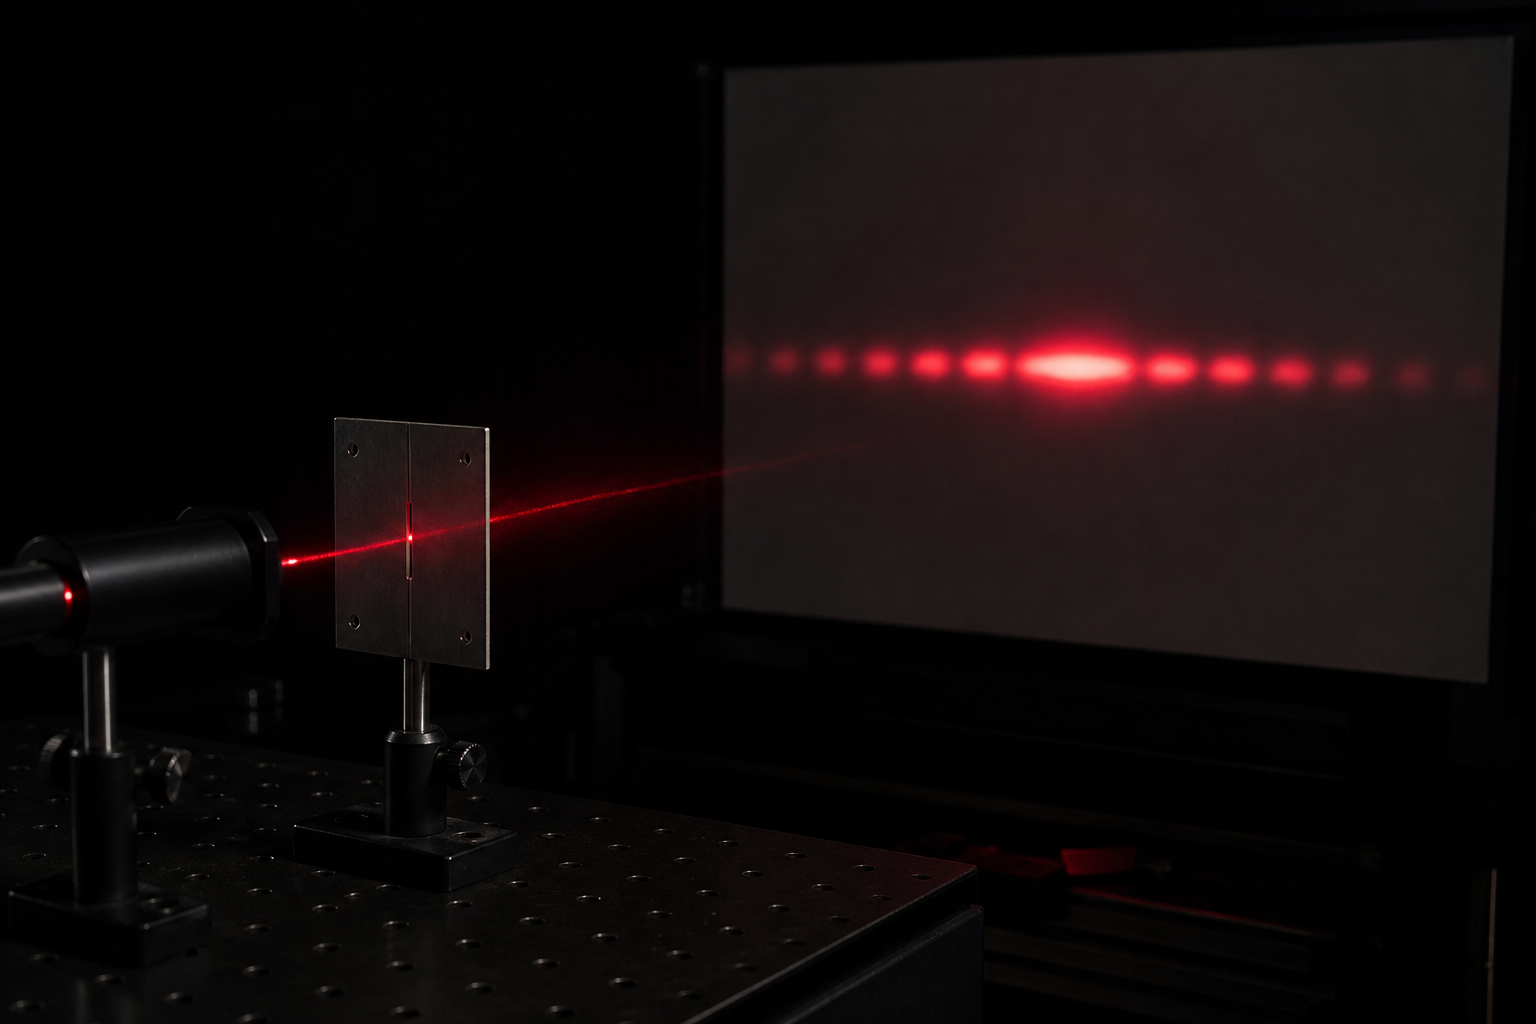
\includegraphics[width=0.58\linewidth]{images/book4/ai/b4-22-slit-diffraction-pattern.png}

{\small Un faisceau laser à travers une fente étroite~: sur l'écran lointain, la large bande centrale brillante et les maxima latéraux plus faibles et plus étroits de la figure de Fraunhofer.}
\end{omfigure}

\section{Problème~: ce que l'on peut résoudre}

\begin{problem}[{Problème du week-end --- la limite de diffraction à quatre
échelles~: l'œil, un télescope, un microscope, et le faisceau laser qu'il
faut nettoyer avant de s'en servir}]
\label{pb:b2:diffraction:1}

\medskip
\noindent\textbf{Partie I --- L'œil.}
Pupille $D = \qty{3}{mm}$ le jour, \qty{7}{mm} la nuit~; $\lambda = \qty{550}{nm}$~; les
cônes de la rétine sont distants de \qty{2}{\micro m} à la fovéa, la distance focale
de l'œil vaut \qty{17}{mm}.
\begin{enumerate}
  \item Rayon angulaire de la \omterm{prop:b2:diffraction:airy}{tache d'Airy} le jour~; son rayon linéaire sur
        la rétine~; comparer à l'espacement des cônes --- la rétine est-elle
        accordée à l'optique~?
  \item Plus petite séparation de deux points résolus à \qty{25}{cm}~; à
        \qty{10}{m}~; peut-on lire un texte de \qty{1}{mm} à bout de bras~?
  \item La nuit la pupille s'ouvre à \qty{7}{mm}~: limite de \omterm{def:b2:diffraction:huygens}{diffraction} alors~;
        pourquoi la vision se dégrade-t-elle néanmoins (aberrations du
        cristallin à pleine ouverture, bâtonnets plus grossiers que les cônes)~?
  \item Deux phares d'automobile distants de \qty{1.5}{m}~: distance à laquelle ils se fondent
        en une seule lumière.
  \item Un trou de \qty{1}{mm} tenu devant l'œil~: que fait la \omterm{def:b2:diffraction:huygens}{diffraction},
        et pourquoi un trou d'épingle aide-t-il néanmoins un œil myope
        (profondeur de champ)~?
\end{enumerate}

\medskip
\noindent\textbf{Partie II --- Le télescope.}
Un télescope de \qty{1}{m}, $f = \qty{10}{m}$, avec une caméra à pixels de \qty{10}{\micro m}~;
$\lambda = \qty{550}{nm}$.
\begin{enumerate}[resume]
  \item Limite de \omterm{def:b2:diffraction:huygens}{diffraction} en secondes d'arc~; rayon d'Airy sur le
        détecteur~; nombre de pixels par \omterm{prop:b2:diffraction:airy}{tache d'Airy}.
  \item L'atmosphère brouille les images à \qty{1}{''}~: quelle part de la
        résolution du télescope est perdue~? Diamètre de télescope pour lequel
        la limite de \omterm{def:b2:diffraction:huygens}{diffraction} égale le seeing.
  \item L'optique adaptative corrige l'atmosphère à \qty{2.2}{\micro m}~:
        limite de \omterm{def:b2:diffraction:huygens}{diffraction} là~; pourquoi est-ce plus facile dans l'infrarouge~?
  \item Une étoile double dont les composantes sont distantes de \qty{0.15}{''}~: résolue avec
        l'optique adaptative à \qty{2.2}{\micro m}~? À \qty{550}{nm} depuis l'espace~?
  \item La Lune est à \qty{3.8e5}{km}~: plus petit cratère que ce télescope
        pourrait résoudre (\omterm{def:b2:diffraction:huygens}{diffraction} seule)~; et l'empreinte d'un module lunaire
        (\qty{4}{m})~?
  \item Pouvoir collecteur du télescope relativement à
        l'œil nocturne (\qty{7}{mm})~; qu'achète-t-il, et quoi non~?
  \item La lumière d'une étoile à travers les quatre bras tenant le
        miroir secondaire~: décrire l'image.
\end{enumerate}

\medskip
\noindent\textbf{Partie III --- Le microscope.}
Objectif d'\omterm{prop:b2:guided-waves:fibre}{ouverture numérique} $\mathrm{NA} = n\sin\alpha = 0.9$ (à sec) ou $1.4$
(à huile), $\lambda = \qty{550}{nm}$~; la distance résolue vaut $0.61\lambda/\mathrm{NA}$.
\begin{enumerate}[resume]
  \item Distance résolue avec chaque objectif~; nombre de paires de traits
        par millimètre.
  \item Une bactérie de \qty{1}{\micro m} à structure interne de
        \qty{0.2}{\micro m}~: que voit-on avec chacun~? Un virus de \qty{0.1}{\micro m}~?
  \item Abbe~: une structure périodique de pas $d$ n'est imagée que si ses
        premiers ordres en $\sin\theta = \lambda/d$ entrent dans l'objectif~: $d$ minimal
        pour $\mathrm{NA} = 1.4$~; comparer à $0.61\lambda/\mathrm{NA}$.
  \item Pourquoi l'huile entre la lame et l'objectif améliore-t-elle la
        résolution~?
  \item L'ultraviolet à \qty{250}{nm} et un microscope électronique à \qty{4}{pm}~:
        distances résolues par la même formule (pour les électrons
        l'\omterm{prop:b2:guided-waves:fibre}{ouverture numérique} pratique vaut \qty{0.01}{})~: comparer.
  \item Une cellule est transparente~: en fond clair son image est vide.
        Expliquer en deux phrases ce que fait la lame de contraste de phase
        placée dans le \omterm{prop:b2:diffraction:fourier}{plan de Fourier} de l'objectif.
\end{enumerate}

\medskip
\noindent\textbf{Partie IV --- Le faisceau.}
Un laser à \qty{532}{nm}, faisceau de \qty{1.5}{mm} de diamètre, doit être élargi à
\qty{30}{mm} et nettoyé.
\begin{enumerate}[resume]
  \item Demi-angle de \omterm{def:b2:diffraction:huygens}{diffraction} du faisceau brut ($\sim1.22\lambda/D$)~; son
        diamètre après \qty{100}{m} sans optique.
  \item Une lentille de $f_1 = \qty{10}{mm}$ le focalise~: diamètre de la tache focale~;
        diamètre du trou choisi ($1.5\times$ la tache).
  \item Une seconde lentille de $f_2$ recollimate à \qty{30}{mm}~: $f_2$~; nouvel
        angle de \omterm{def:b2:diffraction:huygens}{diffraction}~; diamètre après \qty{1}{km}.
  \item Une poussière de \qty{100}{\micro m} sur la première lentille diffracte sous quel angle~;
        où cette lumière tombe-t-elle dans le plan du trou, et que lui
        arrive-t-il~?
  \item Le trou laisse passer $99\%$ d'un faisceau gaussien~: puissance perdue, et
        où elle va.
  \item Pourquoi le faisceau élargi doit-il être \emph{plus large} pour rester parallèle
        (relier $\lambda/D$ à la distance sur laquelle le faisceau double,
        $\sim D^2/\lambda$)~?
  \item Résumer les quatre limites de ce problème en un tableau~: ouverture,
        longueur d'onde, $\lambda/D$, ce qu'elle limite.
\end{enumerate}
\end{problem}
